\documentclass[journal]{IEEEtran}
\usepackage[T1]{fontenc}
\usepackage{amsmath,amssymb,amsfonts}
\usepackage{graphicx}
\usepackage{booktabs}
\usepackage{url}
\usepackage{cite}
\usepackage{array}
\usepackage{multirow}
\interdisplaylinepenalty=2500
\hyphenation{op-tical net-works semi-conduc-tor}

\begin{document}

\title{Fragile Authentication of PDF Signatures via Bit-Exact Quantization Index Modulation on Vector Geometry}

\author{Yaroslav~V.~Baienko%
\thanks{Manuscript received October 23, 2026. The author is an independent researcher (Attorney-at-Law, Legal Engineer \& Applied Cryptography Researcher), Kyiv, Ukraine (ORCID: 0009-0006-7498-2133). A preprint is archived on Zenodo (concept DOI 10.5281/zenodo.23429017); a Ukrainian patent application (a 2026 06266) covers the sealing method.}}

\markboth{IEEE Transactions on Information Forensics and Security,~Vol.~XX,~No.~X,~2026}%
{Baienko: Fragile Authentication of PDF Signatures via Bit-Exact QIM on Vector Geometry}

\maketitle

\begin{abstract}
A PDF signature verifies the bytes it covers, not the page a human sees. The visible layer---seals, stamps and logos---is typically not cryptographically bound to the signed content, so a document can present a valid signature next to altered or transplanted visual material. We study a fragile-authentication watermarking approach that closes this gap at the rendering level: the digest of the signed document is embedded, bit-exactly, into the geometry of the visible seal itself, so the mark a person sees is also the mark that is verified. The carrier is a planar incidence configuration of nine triangles (27 scalar degrees of freedom); the payload uses keyed dithered quantization index modulation (QIM) over an integer coordinate lattice with an exact IEEE-754 rounding argument, and a disjoint carrier degree of freedom carries a per-recipient identifier for leak attribution. No external QR or barcode symbol is added. We evaluate on a corpus of 60 documents produced by LibreOffice, Typst and Chromium print pipelines, each in native, flattened and print-scan-simulated variants (180 PDFs), plus ten public real-world documents. On 1{,}800 stamped PDFs the 266-bit payload is recovered exactly, survives 8-decimal re-serialisation, fails closed at 7 decimals, and any edited payload coordinate is detected; flattening destroys the vector carrier and therefore fails closed. Baselines re-implemented on the same carrier expose a capacity--distortion trade-off rather than a single winner. Two implementation facts are stated explicitly: the PDF writer must preserve at least nine decimal places, and the verifier must parse coordinates as text---drawing APIs that store 32-bit floats destroy a $1.8\times10^{-8}$~pt lattice. The method complements, and does not replace, PAdES/eIDAS signatures.
\end{abstract}

\begin{IEEEkeywords}
fragile watermarking, quantization index modulation, vector graphics, PDF signatures, document authentication.
\end{IEEEkeywords}

\section{Introduction}
A signed PDF can be \emph{valid} and still mislead. The signature covers a byte range; the visual seal is an image or a vector drawing that the signature does not necessarily cover, and incremental updates or flattened copies live outside the signed bytes. The literature on PDF signature attacks documents hidden content \cite{mainka2021} and signature spoofing \cite{mladenov2019}, and document workflows add a third problem: a data room can hand every recipient a visually identical copy, so a leak cannot be attributed.

This paper asks a watermarking question rather than a cryptographic one: can a fragile mark be carried by the visible layer itself, so that (i) the mark is exactly recoverable from the rendered page, (ii) any modification of the mark is detected, and (iii) the mark identifies the recipient copy? The answer explored here is a bit-exact QIM payload embedded in the coordinates of a vector seal. The word \emph{fragile} is deliberate: the goal is not robustness to editing but detection of it.

The contributions are: (1) a bit-exact fragile payload in vector geometry with an exact rounding bound; (2) a carrier that uses the seal itself, so removing or transplanting the seal breaks verification; (3) a disjoint recipient channel; and (4) an evaluation protocol with same-carrier baselines, three document generators, flattened and print-scan variants, a carrier ablation, and a public real-world anchor set. Section~\ref{sec:related} positions the work; Section~\ref{sec:model} states the model; Section~\ref{sec:method} describes the method; Section~\ref{sec:eval} reports the evaluation; Section~\ref{sec:security} gives the attack matrix and the limits of the security argument; Sections~\ref{sec:validity}--\ref{sec:conclusion} discuss validity, reproducibility and limitations.

\section{Related Work}\label{sec:related}
\subsection{Fragile versus robust watermarking}
Robust watermarking aims to survive processing; fragile watermarking aims to detect it. Our work belongs to the second class and is therefore not comparable to robust schemes on bit-error rate under compression---the meaningful axes are exact recovery, distortion and detection. The QIM family \cite{chen2001,eggers2003,perez2004} supplies the lattice; spread-spectrum schemes \cite{cox1997} and early data-hiding constructions \cite{bender1996} supply the historical contrast. Watermarking security analysis \cite{cayre2005} and QIM steganalysis \cite{yang2018} frame what a keyed dither can and cannot promise.

The QIM literature is mature on rate--distortion: dither modulation, distortion-compensated QIM and spread-transform variants trade rate against distortion under an additive-noise model \cite{chen2001,eggers2003}. Our setting differs in two ways. First, the channel is fragile: the verifier must reject any change, so there is no noise budget to optimise against and the relevant question is exactness, not robustness. Second, the host is a vector drawing whose coordinates are serialised as decimal text, so the lattice step must survive decimal formatting and parsing, not an analog channel. A formal steganographic-security claim is left out of scope.

\subsection{Reversible data hiding}
Difference expansion \cite{tian2003}, histogram shifting \cite{ni2006} and prediction-error expansion \cite{thodi2007} define the RDH family. On a 27-slot carrier these schemes are capacity-limited, which we report rather than hide; 2D vector-map RDH \cite{wang2014,peng2019} operates on much larger vertex sets, where capacity is not the binding constraint.

\subsection{Vector graphics and PDF watermarking}
Fourier-descriptor watermarking of 2D vector graphics \cite{doncel2007}, blind vector-graphics schemes \cite{li2003,hou2014}, polar-coordinate vector-data watermarking \cite{mouhamed2012} and mesh-spectral maps \cite{ohbuchi2003} are the closest carrier-level relatives. PDF watermarking itself has been studied in \cite{hatoum2018}, and print-scan resilience in \cite{he2005}. Our carrier is unusual in that the mark is a \emph{visible seal}, not a hidden embedding in an existing drawing; this is what makes the transplant attack meaningful.

\subsection{PDF signature security and standards}
Shadow attacks \cite{mainka2021}, signature spoofing \cite{mladenov2019}, certification attacks \cite{rohlmann2021} and practical decryption exfiltration \cite{muller2019} establish the threat model. Standards \cite{iso32000,etsipades,eidas} define what a compliant signature does and does not cover. Our method does not change the signature; it makes the visible layer that the signature leaves uncovered tamper-evident.

\subsection{Geometric background and visible seals}
The nine-triangle incidence configuration has been studied as a mathematical object
\cite{kulaichev1984,huet2002}, and projective incidence algebra is standard
\cite{richtergebert2011}; the paper uses the configuration only as a stabilised carrier and does not
claim a new geometric theorem. Floating-point exactness follows the standard treatment
\cite{muller2018}. A related industrial idea is the visible digital seal: a QR or bar-code symbol
printed next to a document and bound to its content. Such a seal is an \emph{external} symbol that
can be detached or replaced; the present work removes the symbol and lets the drawing itself carry
the payload, which is what makes the transplant attack meaningful.

\subsection{Commitments, fingerprinting, terminology}
Vector commitments \cite{catalano2013,libert2016} and traitor tracing \cite{boneh1999,tardos2008} are related but not claimed here: the construction is a watermark, not a commitment scheme, and the recipient channel is attribution, not collusion-resistant tracing. The paper deliberately avoids ``vector commitment'' and ``traitor tracing'' as descriptions of its own mechanism.

\subsection{What is new, and what is not}
Table~\ref{tab:families} positions the families; the paper does not claim a new modulation family: QIM, dither modulation and the capacity--distortion view are classical \cite{chen2001,eggers2003,perez2004}, and RDH \cite{tian2003,ni2006,thodi2007} and vector-graphics watermarking \cite{doncel2007,li2003,hou2014} are established. The claim is narrower: a \emph{visible seal} can carry a 256-bit digest bit-exactly, which turns a fragile watermark into a signature-to-rendering binding; the same carrier provides a geometric invariant and a disjoint recipient channel; and the implementation precondition (nine-decimal writers, text-level parsing) is made explicit. The paper does not claim cryptographic security from a watermarking argument and does not claim robustness.

\begin{table}[t]
\centering
\footnotesize
\caption{Positioning against watermarking families.}
\label{tab:families}
\begin{tabular}{@{}p{1.55cm}p{1.25cm}p{1.35cm}p{1.55cm}@{}}
\toprule
Family & Purpose & Carrier & Optimises \\
\midrule
Spread spectrum \cite{cox1997} & robustness & pixels/coeff. & survival \\
QIM/dither \cite{chen2001,eggers2003,perez2004} & rate--distortion & scalar samples & capacity at distortion \\
RDH \cite{tian2003,ni2006,thodi2007,wang2014,peng2019} & reversibility & pixels/vertices & exact cover recovery \\
Vector graphics \cite{doncel2007,li2003,hou2014,mouhamed2012} & robustness & 2D geometry & survival under rescaling \\
PDF marking \cite{hatoum2018} & marking & text/objects & blind detection \\
This work & fragility & visible seal geometry & bit-exact digest recovery \\
\bottomrule
\end{tabular}
\end{table}

\section{System Model and Notation}\label{sec:model}
We consider a document $d$ with a canonical byte representation and a visible seal $S$ drawn as a planar collection of triangles. The issuer computes a 256-bit digest $h=H(d)$ and a 10-bit recipient word $r$, and embeds $(h,r)$ into the seal geometry with a secret key $k$. A verifier receives a PDF and a claimed digest (from the same document) and returns a state in $\{\text{valid},\text{modified},\text{absent}\}$. The carrier is described by 27 scalar slots $\mathbf{s}=(s_1,\dots,s_{27})$ in page coordinates. Table~\ref{tab:notation} lists the notation.

\begin{table}[t]
\centering
\footnotesize
\caption{Notation.}
\label{tab:notation}
\begin{tabular}{@{}ll@{}}
\toprule
Symbol & Meaning \\
\midrule
$d$, $h=H(d)$ & document and its 256-bit digest \\
$r$ & 10-bit recipient identifier \\
$\mathbf{s}$ & 27 carrier slots in page coordinates \\
$\delta(w)$ & lattice shift for a 10-bit word, step $18$~npt \\
$\pi_K$, $d_K$ & keyed slot permutation and word dither \\
valid/modified/absent & verifier output states \\
\bottomrule
\end{tabular}
\end{table}

\section{Threat Model and Requirements}
The adversary can (a) edit the PDF content stream, (b) re-serialise coordinates at reduced precision, (c) flatten the page to a raster image, (d) transplant a visual seal from another document, and (e) redistribute a copy. The verifier knows the canonical seal geometry and the document digest. We state four requirements: \emph{exactness} (the 256-bit digest is recovered bit for bit); \emph{fragility} (any edit of a payload coordinate changes the recovered digest); \emph{fail-closed} behaviour (when the vector layer is absent, the verifier refuses rather than accepts); and \emph{attribution} (a recipient identifier is carried independently of the digest).

The threat model is deliberately weaker than a cryptographic one: we do not claim that an adversary cannot produce a new document with a new seal, only that an edited or transplanted seal is detectable relative to a known document digest.

\section{Method}\label{sec:method}
\subsection{Carrier and degrees of freedom}
The seal is drawn as nine triangles. Each triangle contributes three degrees of freedom---base line, apex, half-width---for 27 scalar slots. Because the triangles share a construction centre, the bilateral relation $lx+rx=2cx$ and the common centre are geometric invariants, checked independently of the payload. A generic 27-vertex polyline and a $9\times3$ grid are used as ablations: they carry the same 27 slots at the same distortion, but have no such invariant (Fig.~\ref{fig:carriers}).

\begin{figure*}[t]
\centering
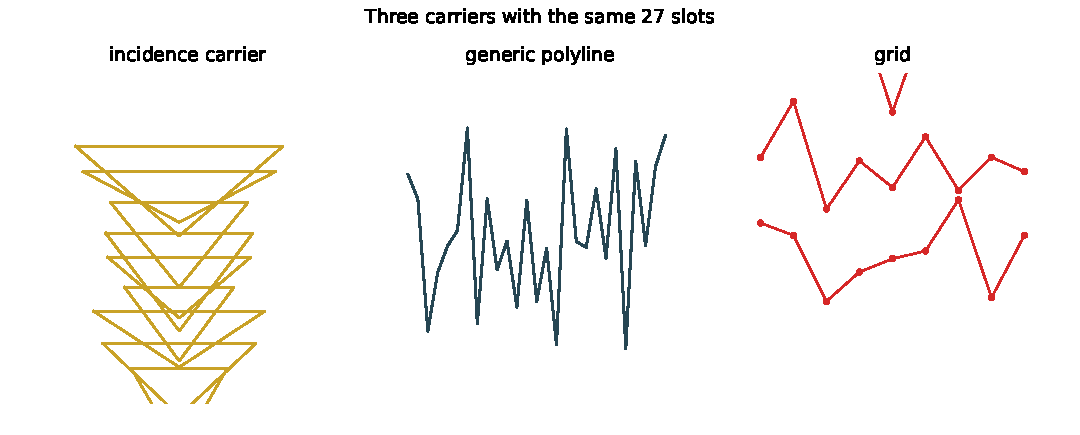
\includegraphics[width=0.9\textwidth]{figures/fig_carriers.pdf}
\caption{The three carriers used in the ablation. All three carry the same 27 slots at the same distortion; only the incidence configuration (left) has the bilateral and common-centre invariants.}
\label{fig:carriers}
\end{figure*}

\subsection{Bit-exact word mapping}
A 256-bit digest is split into 26 words of 10 bits; the 27th word carries a 10-bit recipient identifier. A 10-bit word $w$ maps to the coordinate shift
\begin{equation}
\delta(w)=(18w-9207)\times10^{-9}~\text{pt},
\end{equation}
i.e.\ a multiple of $18$~npt $=1.8\times10^{-8}$~pt, with $w\in[0,1023]$.

\subsection{Exactness argument}
At coordinates of the order of $3\times10^{2}$~pt the IEEE-754 double spacing is $2^{-52}\times2^{9}\approx1.1\times10^{-13}$~pt, more than four orders of magnitude below the step, so every lattice point is exactly representable and a recovered word has no rounding ambiguity. Re-serialising a coordinate with eight decimal places rounds it to the nearest $10^{-8}$~pt, an error of at most $5\times10^{-9}$~pt, below half a step ($9\times10^{-9}$~pt); seven decimal places (error up to $5\times10^{-8}$~pt) exceeds half a step and destroys the word.

\subsection{Keyed dither and recipient channel}
A key derives a permutation $\pi_K$ of the 27 slots and a word-level dither $d_K$. The digest words are dithered and permuted before embedding, and the recipient word is placed in the remaining slot. The dither does not change the lattice spacing, so exactness is preserved; it changes which physical slot carries which word, so an unkeyed reader cannot align the payload with the geometry.

\subsection{Encoding and decoding}
\textbf{Encode} $(d,r,k)$: (1) $h\leftarrow H(d)$; split $h$ into 26 ten-bit words $w_1..w_{26}$; append $w_{27}\leftarrow r$. (2) derive $(\pi_K,d_K)$ from the key and a document nonce; $v_i\leftarrow(w_{\pi_K(i)}+d_K(i))\bmod 1024$. (3) $s'_i\leftarrow s_i+\delta(v_i)$ for $i=1..27$. (4) write the path operators with nine decimals; return the stamped PDF and $h$.

\textbf{Decode} $(PDF,h,k)$: (1) parse the content stream as text; locate the carrier path by marker colour/width. (2) reconstruct $s'_i$ from the path; $v_i\leftarrow\delta^{-1}(s'_i-s_i)$; undo $(\pi_K,d_K)$. (3) reassemble the 27 words; compare words 1--26 with $H(d)$; return the recipient word. (4) if the path is absent return \emph{absent}; if comparison fails return \emph{modified}; else \emph{valid}.

\subsection{Implementation precondition}
The carrier must be written with at least nine decimal places. Common PDF writers emit five decimals, which destroys the $1.8\times10^{-8}$~pt lattice; the reference implementation therefore injects path operators into the content stream directly rather than using a drawing API. The verifier must parse the numbers as text, because drawing APIs that store coordinates as 32-bit floats lose the lattice as well.

\subsection{Complexity and deployment notes}
Stamping is linear in the number of pages and constant in payload length: the carrier is a fixed 27-slot path, so the cost is one content-stream edit per page. On the development machine stamping costs about 1.05~ms and verification about 0.33~ms per page. A deployment assigns 10-bit recipient identifiers, which bounds one key epoch to 1{,}024 tracked copies; larger deployments rotate the key or extend the identifier space.

\section{Evaluation}\label{sec:eval}
\subsection{Corpus}
Sixty synthetic documents are generated by three independent pipelines: LibreOffice (DOCX to PDF), Typst, and Chromium print-to-PDF. Each document exists in three variants: \emph{native}, \emph{flattened} (300~dpi raster re-wrapped as an image-only PDF) and \emph{print-scan simulated} (200~dpi, Gaussian blur, sensor noise, JPEG q=70). The corpus contains 180 PDFs (51.1~MB) with a SHA-256 manifest. Ten unique public real-world documents (whitepapers, manuscript PDFs and patent description PDFs; no client data) are used as anchors.

\subsection{Protocol}
For each document and seed, the payload is $H(\text{doc\_sha}\Vert\text{seed})$; the 266-bit payload is embedded with keyed QIM, and the stamped PDF is attacked in the content stream (8/7-decimal truncation, payload-coordinate edit, centre-line edit) or flattened. The experiment runs 60 documents $\times$ 30 seeds (1{,}800 samples), plus 360 samples on flattened/print-scan inputs, plus an ablation over three carriers and keyed/unkeyed embedding, plus 100 samples on the real-world anchors.

\subsection{Metrics and attack parameters}
\emph{Geometric RMSE} is the root-mean-square coordinate change over the 27 slots; \emph{PSNR$_{\text{geom}}$} is $20\log_{10}(300/\text{RMSE})$ with the 300~pt geometry normalisation. \emph{Exact} is one only if all 27 recovered words equal the embedded words. \emph{Detection} is one if the recovered words differ from the expected words (payload edit) or if a geometric invariant fails (centre-line edit). Truncation rewrites every coordinate number in the carrier path to 8 or 7 decimal places. The payload-coordinate edit changes one coordinate by $10^{-4}$~pt; the centre-line edit changes a non-payload coordinate by $0.5$~pt. Flattening replaces the page by a 300~dpi raster image.

\subsection{Results}
Fig.~\ref{fig:capdist} and Tables~\ref{tab:main}--\ref{tab:baselines} summarise the results. On the main experiment, the 266-bit payload is recovered exactly in 100\% of 1{,}800 samples (mean geometric RMSE $5.31\times10^{-6}$~pt, PSNR$_{\text{geom}}=155.1$~dB), survives 8-decimal truncation in 100\% of samples, is detected at 7-decimal truncation in 100\%, detects every payload-coordinate edit, and fails closed on every flattened page. The per-generator breakdown is in Table~\ref{tab:pergen} and Fig.~\ref{fig:pergen}; the ten public real-world anchors reproduce the same behaviour (100 samples).

\begin{figure}[t]
\centering
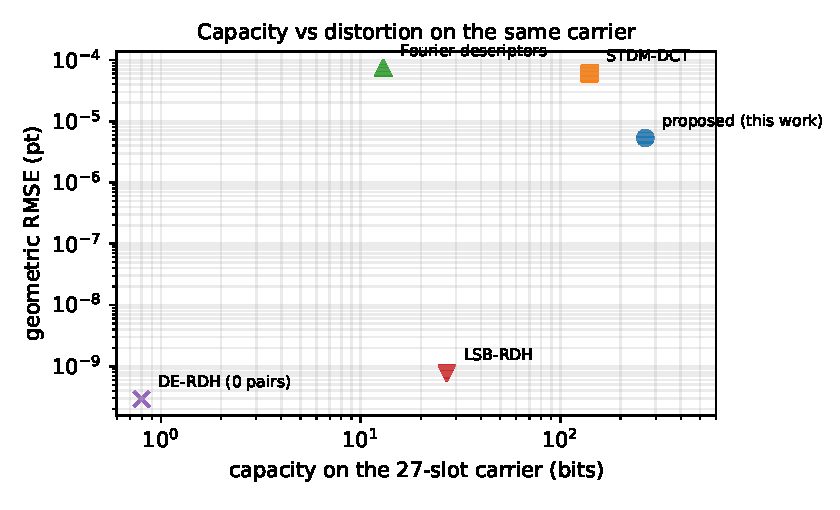
\includegraphics[width=\columnwidth]{figures/fig_capacity_distortion.pdf}
\caption{Capacity versus geometric distortion on the same 27-slot carrier. The proposed payload carries 266 bits at RMSE $5.3\times10^{-6}$~pt; capacity-limited baselines are marked at their maximum capacity.}
\label{fig:capdist}
\end{figure}

\begin{table}[t]
\centering
\footnotesize
\caption{PDF-level results on 60 native documents $\times$ 30 seeds.}
\label{tab:main}
\begin{tabular}{@{}lccc@{}}
\toprule
Metric & Result & 95\% CI & Samples \\
\midrule
Exact digest recovery & 100\% & 0.00 & 1800/1800 \\
Survives 8-decimal truncation & 100\% & 0.00 & 1800/1800 \\
Detected at 7-decimal truncation & 100\% & 0.00 & 1800/1800 \\
Edited payload coordinate detected & 100\% & 0.00 & 1800/1800 \\
Flattening removes the carrier & 100\% & 0.00 & 1800/1800 \\
\bottomrule
\end{tabular}
\end{table}

\begin{table}[t]
\centering
\footnotesize
\caption{Per-generator breakdown of the main experiment.}
\label{tab:pergen}
\begin{tabular}{@{}lcccc@{}}
\toprule
Generator & Samples & Exact & Detected at 7 dec. & RMSE (pt) \\
\midrule
LibreOffice & 600 & 100\% & 100\% & $5.30\times10^{-6}$ \\
Typst & 600 & 100\% & 100\% & $5.33\times10^{-6}$ \\
Chromium & 600 & 100\% & 100\% & $5.29\times10^{-6}$ \\
\bottomrule
\end{tabular}
\end{table}

\begin{table}[t]
\centering
\footnotesize
\caption{Carrier ablation: all carriers carry the same 27 slots.}
\label{tab:ablation}
\begin{tabular}{@{}llccc@{}}
\toprule
Carrier & Keyed & Exact & Trunc-8 & Centre edit detected \\
\midrule
Sri Yantra & yes & 100\% & 100\% & 100\% \\
Sri Yantra & no & 100\% & 100\% & 100\% \\
Generic polyline & yes & 100\% & 100\% & 0\% \\
Generic polyline & no & 100\% & 100\% & 0\% \\
Grid & yes & 100\% & 100\% & 0\% \\
Grid & no & 100\% & 100\% & 0\% \\
\bottomrule
\end{tabular}
\end{table}

\begin{figure}[t]
\centering
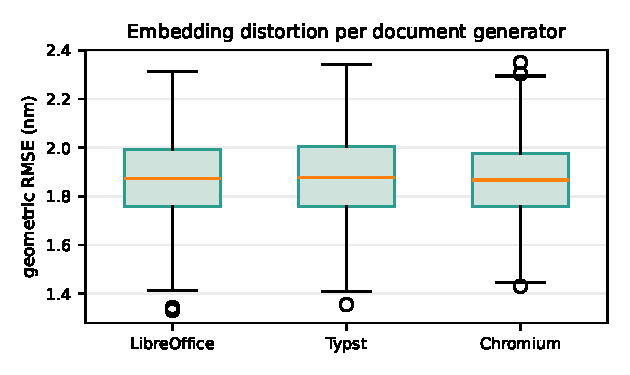
\includegraphics[width=\columnwidth]{figures/fig_pergen.pdf}
\caption{Embedding distortion per document generator (geometric RMSE in nanometres; medians 1.87--1.88~nm).}
\label{fig:pergen}
\end{figure}

\subsection{Precision precondition in practice}
The exactness argument predicts a cliff between eight and seven decimal places. The measurement matches the prediction: exact recovery is 100\% at 9 and 8 decimals and drops to 0\% at 7 and 6 decimals (Fig.~\ref{fig:precision}). This is a property of the pipeline after sealing, not of the document generator: the corpus generators themselves emit between three and six decimal places (Table~\ref{tab:writers}), and the carrier is injected after generation. A production document-management system that re-writes coordinates with fewer than eight decimals destroys the mark; the verifier reports \emph{absent} rather than \emph{valid} (fail-closed).

\begin{figure}[t]
\centering
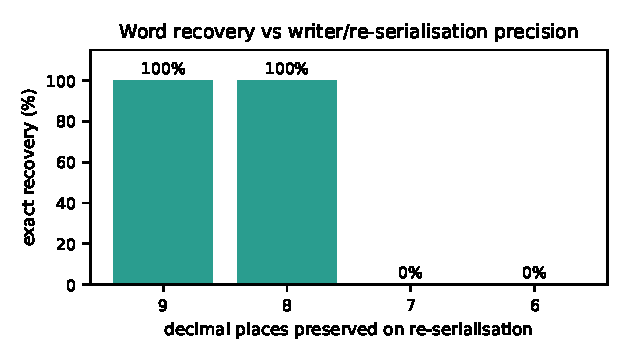
\includegraphics[width=\columnwidth]{figures/fig_precision.pdf}
\caption{Word recovery versus the number of decimal places preserved on re-serialisation.}
\label{fig:precision}
\end{figure}

\begin{table}[t]
\centering
\footnotesize
\caption{Writer precision of the corpus generators.}
\label{tab:writers}
\begin{tabular}{@{}lcc@{}}
\toprule
Generator & Avg.\ decimals & Carrier exact after injection \\
\midrule
LibreOffice DOCX to PDF & 3.16 & 100\% \\
Chromium print-to-PDF & 5.27 & 100\% \\
Typst & 5.76 & 100\% \\
\bottomrule
\end{tabular}
\end{table}

\subsection{Public real-world anchors}
Ten unique public project documents were stamped and attacked under the same protocol (10 seeds each, 100 samples). Results match the synthetic corpus: exact recovery in 100\% of samples, 8-decimal re-serialisation survives, 7-decimal re-serialisation and payload edits are detected, and flattening removes the carrier. Mean geometric RMSE is $5.32\times10^{-6}$~pt (PSNR$_{\text{geom}}=155.0$~dB).

\subsection{Capacity, performance and storage}
Capacity is per visible seal: 266 bits over a seal of about $126\times185$~pt ($23{,}227$~pt$^2$),
i.e. $0.0115$~bit/pt$^2$; no document-wide capacity claim is made. Stamping is linear in the number
of pages and constant in payload length. On the development machine, stamping costs about
1.05~ms per page and verification about 0.33~ms per page, dominated by PDF parsing and stream
rewriting rather than by the embedding arithmetic. The carrier path is small and, after stream
compression, adds only a few bytes to the file in our samples; memory use is proportional to one
page at a time.

\subsection{Same-carrier baselines}
STDM-DCT, Fourier-descriptor and LSB-RDH embedding were re-implemented on the same carrier at slot level and re-run at the PDF level (20 documents $\times$ 10 seeds, 600 samples). The comparison is a capacity--distortion--fragility frontier, not a ranking (Table~\ref{tab:baselines}). Only the proposed scheme reaches a 266-bit digest on 27 slots; STDM reaches 140 bits at higher distortion; Fourier descriptors reach 13 bits; LSB reaches 27 bits at negligible distortion but is destroyed by 8-decimal re-serialisation.

\begin{table}[t]
\centering
\footnotesize
\caption{Same-carrier baselines (PDF level, 600 samples).}
\label{tab:baselines}
\begin{tabular}{@{}lcccc@{}}
\toprule
Method & Capacity & RMSE (pt) & Exact & Exact at 8 dec. \\
\midrule
Proposed (keyed QIM) & 266 & $5.31\times10^{-6}$ & 100\% & 100\% \\
STDM-DCT & 140 & $6.16\times10^{-5}$ & 100\% & 100\% \\
Fourier descriptors & 13 & $7.27\times10^{-5}$ & 100\% & 100\% \\
LSB-RDH & 27 & $7.03\times10^{-10}$ & 100\% & 0\% \\
DE-RDH & 0 & $2.91\times10^{-10}$ & n/a & n/a \\
\bottomrule
\end{tabular}
\end{table}

\subsection{Discussion}
\emph{Why exactness changes the application.} An error-tolerant watermark can carry a few bits and survive processing, but it cannot carry a cryptographic digest: one flipped bit makes the digest meaningless. Exactness is what turns the visible seal into a verifier of the signed bytes. The price is fragility---the mark dies under any change, including innocent re-serialisation---and the paper makes that price explicit rather than hiding it behind a robustness claim.

\emph{What the carrier adds.} With capacity and distortion held fixed, the generic polyline and the grid recover the payload as reliably as the incidence configuration (Table~\ref{tab:ablation}). The difference is the geometric invariant: the incidence construction fixes the triangle centres, so a centre-line edit outside the payload slots is detected even before the digest comparison.

\emph{What the baselines show.} STDM and Fourier-descriptor embedding reach 140 and 13 bits on the same carrier at higher distortion; LSB reaches 27 bits at negligible distortion but is destroyed by 8-decimal re-serialisation.

\section{Attack Matrix and Security Discussion}\label{sec:security}
\begin{table}[t]
\centering
\footnotesize
\caption{Attack matrix.}
\label{tab:attack}
\begin{tabular}{@{}p{2.0cm}p{2.2cm}p{1.0cm}@{}}
\toprule
Attack & Expected outcome & Measured \\
\midrule
Payload-coordinate edit & digest changes, detected & 100\% \\
Centre-line edit & geometry invariant fails & 100\% (incidence only) \\
8-decimal re-serialisation & digest unchanged & 100\% exact \\
7-decimal re-serialisation & digest changes, detected & 100\% \\
Flattening & carrier absent, fail-closed & 100\% absent \\
Seal transplant & digest mismatch & by construction \\
\bottomrule
\end{tabular}
\end{table}

\begin{table}[t]
\centering
\footnotesize
\caption{Attack taxonomy and residual risk.}
\label{tab:taxonomy}
\begin{tabular}{@{}p{1.55cm}p{1.7cm}p{1.7cm}@{}}
\toprule
Class & Capability & Detection / residual risk \\
\midrule
Stream edit & rewrite path or text & digest mismatch; geometry invariant \\
Precision loss & re-serialise with $d\le7$ decimals & digest mismatch; fail-closed if path lost \\
Geometric edit & move a non-payload coordinate & incidence invariant (Sri Yantra only) \\
Rasterisation & flatten or print-scan & carrier absent, fail-closed; optical channel out of scope \\
Seal transplant & paste a seal from another document & digest mismatch \\
Redistribution & forward a sealed copy & recipient word attribution \\
\bottomrule
\end{tabular}
\end{table}

The construction authenticates the rendering layer, not the cryptographic signature (Tables~\ref{tab:attack} and~\ref{tab:taxonomy}). It does not prevent an attacker from producing a new document with a new valid seal; it makes a transplanted or edited seal detectable relative to a known document digest. The recipient channel provides attribution for a leaked copy; it is not a collusion-resistant fingerprinting code, and traitor-tracing security is not claimed.

\subsection{Assumptions and claims}
\emph{A1}: the verifier knows the canonical seal geometry for the document class. \emph{A2}: the
document digest is known or can be recomputed from the signed bytes. \emph{A3}: the key is secret.
\emph{A4}: the post-sealing pipeline preserves at least nine decimal places.

\emph{P1 (payload-edit detection)}: changing any payload slot changes the recovered word, because
the lattice step exceeds the rounding error by a factor of two and the digest is compared bit for
bit. \emph{P2 (fail-closed)}: if the carrier path is absent, the verifier returns \emph{absent}.
\emph{P3 (attribution)}: with the key, the recovered recipient word equals the embedded word;
without the key, the recovered words are unpredictable to the adversary. These are watermarking
claims, not cryptographic reductions: the paper does not claim that an adversary cannot produce a
new document with a new valid seal, and it does not claim collusion resistance of the recipient
channel.

\section{Threats to Validity}\label{sec:validity}
\emph{Internal validity.} Exactness is deterministic by construction, so the zero-width confidence intervals do not measure real-world variability; the meaningful variation must come from document generators, production PDF writers and physical capture, which this draft only partially exercises.

\emph{External validity.} The corpus is synthetic and generated by three pipelines on one machine; real documents pass through enterprise DMS flattening, print-to-PDF converters, optimisers and archival re-writers whose coordinate serialisation differs. The 8-decimal precondition is a filter that such pipelines may fail.

\emph{Construct validity.} The baselines share the carrier and the distortion metric but not the PDF-level embedding code of the proposed method, which favours the proposed method on implementation maturity; the PDF-level baseline re-runs reduce but do not remove this gap.

\emph{Conclusion validity.} The comparisons are exact-match and distortion measurements with 30 seeds; they are not hypothesis tests about a population of documents.

\section{Ethical Considerations}
The method is intended for document integrity and leak attribution in lawful workflows. Its recipient channel is an attribution mechanism, not a surveillance mechanism. The evaluation uses synthetic documents and public project documents only; no client data and no personal data are processed. A deployment must disclose recipient marking to the parties where the applicable law requires it.

\section{Reproducibility and Declarations}
The corpus builder, carrier layer, attack harness and baseline implementations are versioned with the manuscript; the corpus manifest records a SHA-256 per file and the corpus is regenerated deterministically from a seed. The measured tables are produced by the harness. Code and the corpus manifest are available from the author; the corpus is regenerated by the provided script. A preprint is available at the concept DOI 10.5281/zenodo.23429017. Competing interests: none. Funding: none. The method is covered by a pending Ukrainian patent application (a 2026 06266).

\section{Failure Modes in Deployment}
Three failure modes follow directly from the design. (i) \emph{Precision loss:} any pipeline stage that re-writes coordinates with fewer than eight decimals destroys the word; the verifier fails closed. (ii) \emph{Rasterisation:} flattening removes the vector layer; the verifier reports absent. (iii) \emph{Seal regeneration:} if a verifier is given a new document and a new valid seal, the method has nothing to compare against; it authenticates a seal relative to a known document digest, not the identity of a signer.

\section{Future Work}
Three directions follow. First, a physical print-scan set (phone camera, office scanner) will test the fail-closed claim under real optics rather than simulation. Second, the carrier can be tested against production document-management pipelines that re-write coordinates. Third, the recipient channel can be extended beyond 1{,}024 copies per key epoch at a known capacity cost.

\section{Limitations and Conclusion}\label{sec:conclusion}
The evaluation is a first harness result. The baselines are re-implemented on the same carrier and must be lifted further; the print-scan variant is a simulation, not a physical scanner; the corpus is synthetic; and exactness is deterministic, so the reported confidence intervals are not informative about real-world variability. Capacity numbers are per seal, not per document area. Within these limits the result is consistent and reproducible: 1{,}800 PDF-level samples recover the 266-bit payload exactly, 8-decimal re-serialisation is safe, 7-decimal re-serialisation and any payload edit are detected, and flattening fails closed.

\appendices
\section{Proof Details}
\emph{Lemma 1 (the word map is a bijection).} Write $\delta(w)=(18w-9207)\times10^{-9}$. For integer $w$ the values are distinct because $18w$ is strictly increasing; neighbouring words differ by exactly $18\times10^{-9}$~pt. The decoder computes $n=\mathrm{round}(\delta\cdot10^{9})=18w-9207$ exactly while the coordinate error is below $0.5\times10^{-9}$~pt; then $\mathrm{round}((n+9207)/18)=w$.

\emph{Lemma 2 (eight decimals are sufficient).} Rounding a real coordinate $x$ to $d$ decimal places yields $|x-\mathrm{round}_d(x)|\le0.5\times10^{-d}$~pt. For $d=8$ this is at most $5\times10^{-9}$~pt, while half the lattice step is $9\times10^{-9}$~pt; the decoder returns the same word. For $d=7$ the bound is $5\times10^{-8}$~pt, above half a step, so adjacent words can be confused.

\section{Generator Settings}
The corpus is generated with LibreOffice headless (DOCX to PDF, default settings), Typst (A4, 2.2~cm margins) and Chromium print-to-PDF (headless, no header/footer). Flattening uses a 300~dpi raster; the print-scan simulation uses 200~dpi, a Gaussian blur, additive Gaussian sensor noise and JPEG quality 70. All settings are recorded in the corpus builder so the corpus can be regenerated from the published script and seed.

\bibliographystyle{IEEEtran}
\bibliography{references}

\end{document}
